\documentclass[a4paper,UTF8]{article}
\usepackage{ctex}
\usepackage[margin=1.25in]{geometry}
\usepackage{color}
\usepackage{graphicx}
\usepackage{amssymb}
\usepackage{amsmath}
\usepackage{amsthm}
%\usepackage[thmmarks, amsmath, thref]{ntheorem}
\theoremstyle{definition}
\newtheorem*{solution}{Solution}
\newtheorem*{prove}{Proof}
\usepackage{multirow}
\usepackage{url}
\usepackage{enumerate}
\usepackage{algorithm}
\usepackage{algorithmic}
\renewcommand{\algorithmicrequire}{\textbf{Input:}}
\renewcommand{\algorithmicensure}{\textbf{Procedure:}}
\renewcommand\refname{参考文献}

%--

%--
\begin{document}
\title{实验3. 强化学习实践}
\author{MG1733099,周天烁,\url{tianshuo.zhou@smail.nju.edu.cn}}
\maketitle

\section{综述}
    \paragraph*{}
	通过解决Gym为用户提供了一些基础强化学习任环境,如CartPole-v0、MountainCar-v0和Acrobot-v1等,完成强化学习的任务,加深对强化学习的理解。


\section{实验二. }
    \paragraph*{}
    通过连续空间离散化的方式,实现Q-learning算法,并用于求解CartPole-v0、MountainCar-v0和Acrobot-v1三个学习任务。由于三个任务的状态空间都是连续的,所以最直接的方式就是
    将状态空间等分,把每个状态映射到等分的一个个区间里。具体等分方式视任务而定,即调参过程。
    \paragraph*{}
    为了调用统一的函数,对于3个任务,每个任务都是训练2000轮(episode),测试100轮(episode),打印结果为每个每轮测试结果及其均值和标准差。
\subsection{CartPole-v0}
    状态空间有4个维度,等分方式为(1,1,6,5)。实验运行结果如图1所示。
    \begin{center}
    \begin{figure}[H]
          \centering
          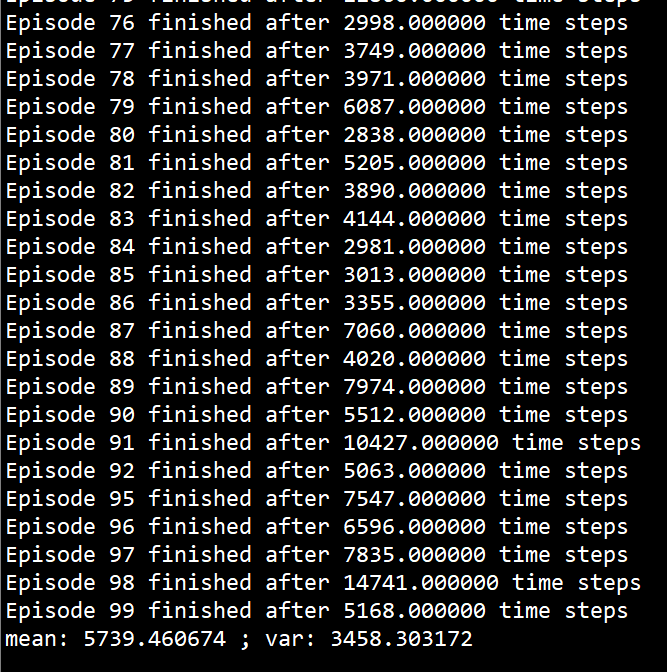
\includegraphics[width=12cm]{1.png}
          \caption{Q-learning:CartPole-v0}
          \label{fig:2.3}
    \end{figure}
    \end{center}
\subsection{MountainCar-v0}
    状态空间有2个维度,等分方式为(20,20)。实验运行结果如图2所示。
    \begin{center}
    \begin{figure}[H]
          \centering
          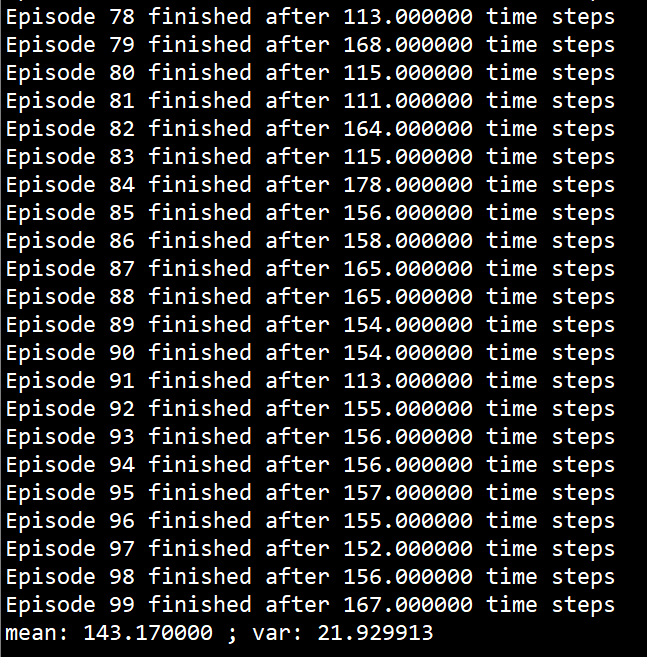
\includegraphics[width=12cm]{2.png}
          \caption{Q-learning:MountainCar-v0}
          \label{fig:2.3}
    \end{figure}
    \end{center}
\subsection{Acrobot-v1}
    状态空间有6个维度,等分方式为(6,6,6,6,6,6)。实验运行结果如图3所示。
    \begin{center}
    \begin{figure}[H]
          \centering
          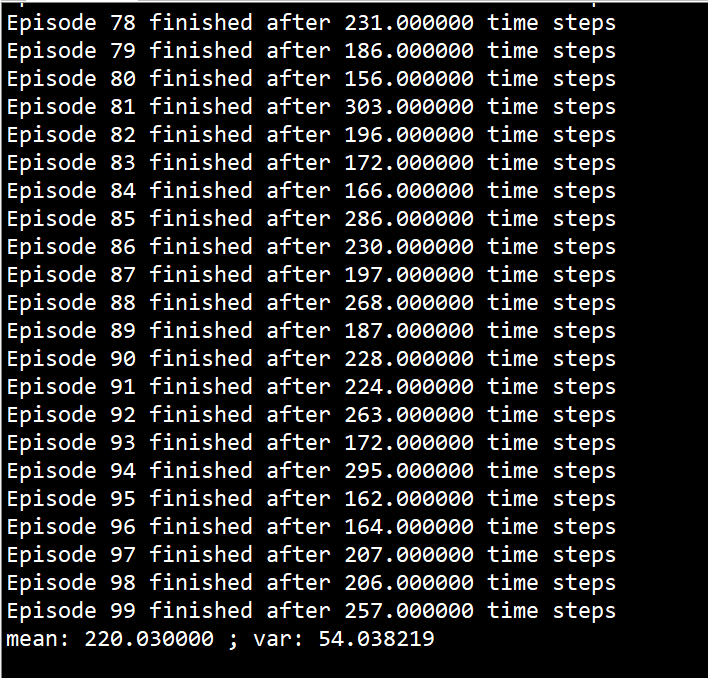
\includegraphics[width=12cm]{3.png}
          \caption{Q-learning:Acrobot-v1}
          \label{fig:2.3}
    \end{figure}
    \end{center}
	
\section{实验三. }
    \paragraph*{}
	利用Deep Q-learning(DQN)算法直接在连续的空间中进行学习,完成CartPole-v0、MountainCar-v0和Acrobot-v1这三个任务,在实验三中我们直接
    在连续空间中学习。DQN 的算法主要是是实现一个Q 函数网络。本实验采用的Q值网络为Multi-layer Perceptron (MLP),通
    过学习一组深度网络参数使Q函数网络的输出近似于真实的Q值。
    
    \subsection{CartPole-v0}
    基本参数和实验二一致,MLP含有一个输入层,一个输出层和两个隐层。训练过程中损失(loss)变化如图4所示,累计奖赏(sum of reward)变化如图5所示。实验运行结果如图6所示。
    \begin{center}
    \begin{figure}[H]
          \centering
          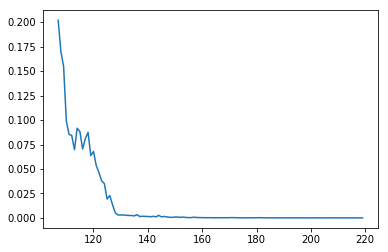
\includegraphics[width=12cm]{5.png}
          \caption{DQN:CartPole-v0 loss曲线}
          \label{fig:2.3}
    \end{figure}
    \end{center}
    \begin{center}
    \begin{figure}[H]
          \centering
          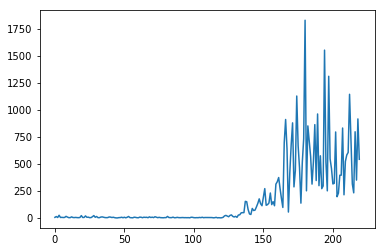
\includegraphics[width=12cm]{6.png}
          \caption{DQN:CartPole-v0 sum of reward曲线}
          \label{fig:2.3}
    \end{figure}
    \end{center}
    \begin{center}
    \begin{figure}[H]
          \centering
          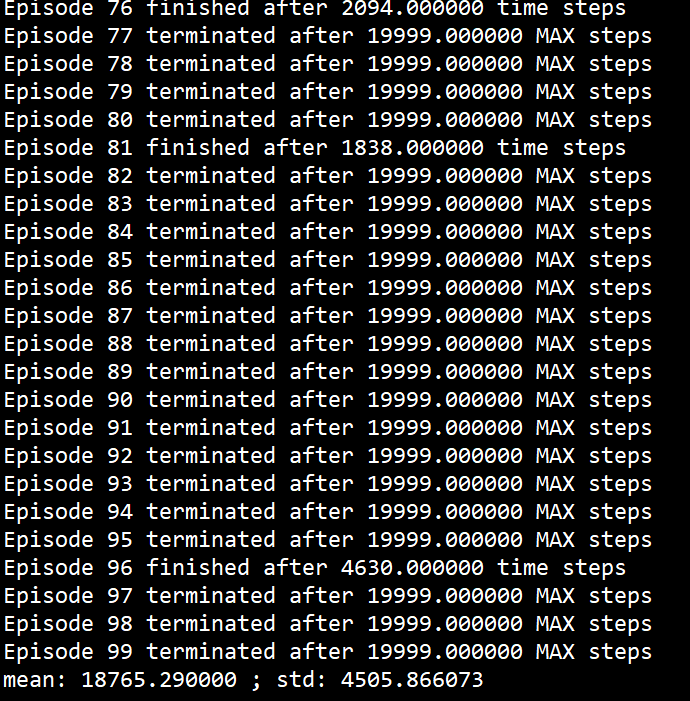
\includegraphics[width=12cm]{4.png}
          \caption{DQN:CartPole-v0}
          \label{fig:2.3}
    \end{figure}
    \end{center}
    \subsection{MountainCar-v0}
    基本参数和实验二一致,MLP含有一个输入层,一个输出层和两个隐层。训练过程中损失(loss)变化如图7所示,累计奖赏(sum of reward)变化如图8所示。实验运行结果如图9所示。
    
    \begin{center}
    \begin{figure}[H]
          \centering
          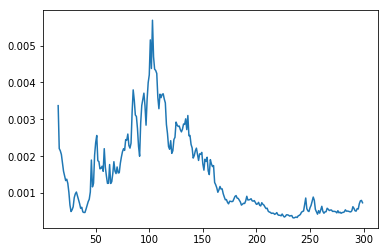
\includegraphics[width=12cm]{7.png}
          \caption{DQN:MountainCar-v0 loss曲线}
          \label{fig:2.3}
    \end{figure}
    \end{center}
    \begin{center}
    \begin{figure}[H]
          \centering
          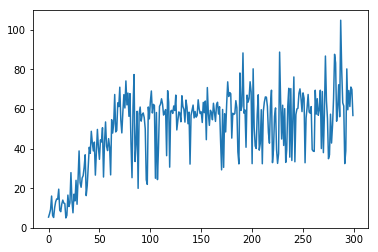
\includegraphics[width=12cm]{8.png}
          \caption{DQN:MountainCar-v0 sum of reward曲线}
          \label{fig:2.3}
    \end{figure}
    \end{center}
    \begin{center}
    \begin{figure}[H]
          \centering
          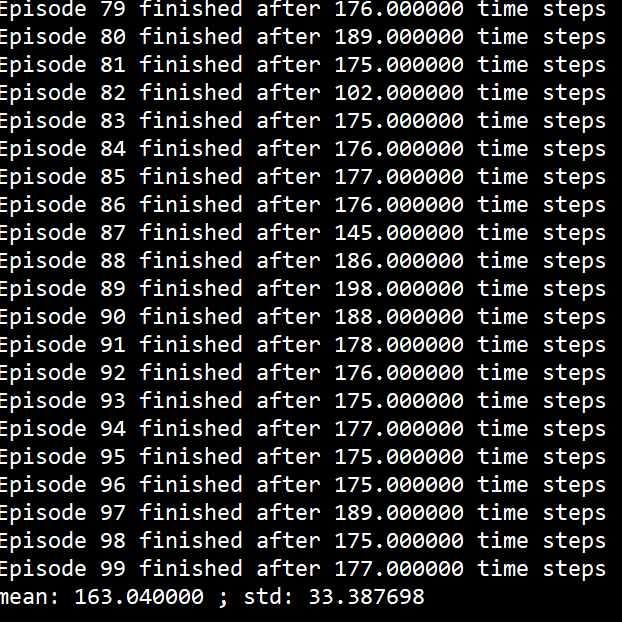
\includegraphics[width=12cm]{9.png}
          \caption{DQN:MountainCar-v0}
          \label{fig:2.3}
    \end{figure}
    \end{center}
    
    \subsection{Acrobot-v1}
    基本参数和实验二一致,MLP含有一个输入层,一个输出层和两个隐层。训练过程中损失(loss)变化如图10所示,累计奖赏(sum of reward)变化如图11所示。实验运行结果如图12所示。

    \begin{center}
    \begin{figure}[H]
          \centering
          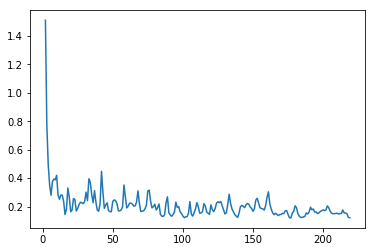
\includegraphics[width=12cm]{22.png}
          \caption{DQN:Acrobot-v1 loss曲线}
          \label{fig:2.3}
    \end{figure}
    \end{center}
    \begin{center}
    \begin{figure}[H]
          \centering
          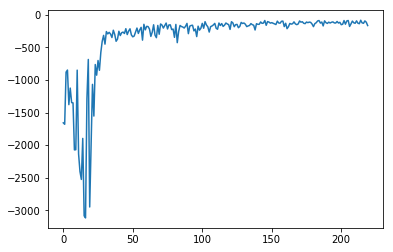
\includegraphics[width=12cm]{23.png}
          \caption{DQN:Acrobot-v1 sum of reward曲线}
          \label{fig:2.3}
    \end{figure}
    \end{center}
    \begin{center}
    \begin{figure}[H]
          \centering
          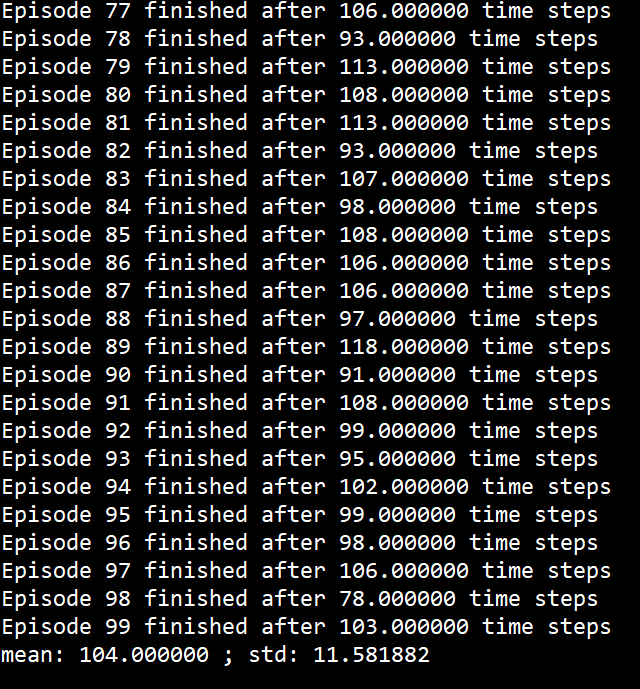
\includegraphics[width=12cm]{21.png}
          \caption{DQN:Acrobot-v1}
          \label{fig:2.3}
    \end{figure}
    \end{center}
    
	
\section{实验四. }
	\paragraph*{}
	对实验三的Deep Q-learning(DQN)算法进行改进。唯一的区别是Q值网络函数的更新方式不同,其它参数基本和实验三相同。

    \subsection{CartPole-v0}
    训练过程中损失(loss)变化如图13所示,累计奖赏(sum of reward)变化如图14所示。实验运行结果如图15所示。
    \begin{center}
    \begin{figure}[H]
          \centering
          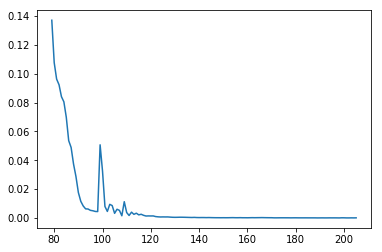
\includegraphics[width=12cm]{29.png}
          \caption{MyImprovedDQN:CartPole-v0 loss曲线}
          \label{fig:2.3}
    \end{figure}
    \end{center}
    \begin{center}
    \begin{figure}[H]
          \centering
          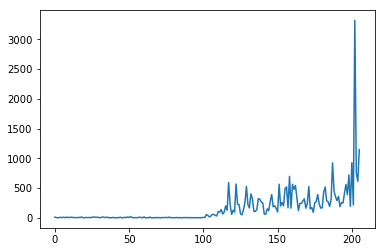
\includegraphics[width=12cm]{30.png}
          \caption{MyImprovedDQN:CartPole-v0 sum of reward曲线}
          \label{fig:2.3}
    \end{figure}
    \end{center}
    \begin{center}
    \begin{figure}[H]
          \centering
          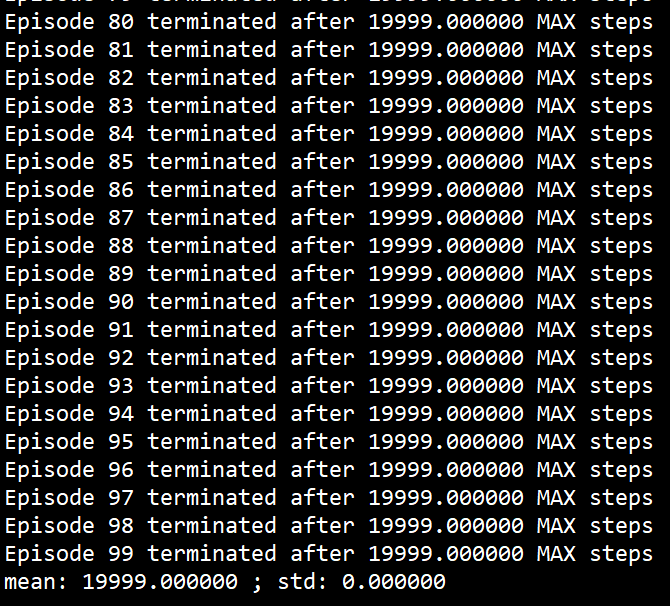
\includegraphics[width=12cm]{28.png}
          \caption{MyImprovedDQN:CartPole-v0}
          \label{fig:2.3}
    \end{figure}
    \end{center}
    \subsection{MountainCar-v0}
    训练过程中损失(loss)变化如图16所示,累计奖赏(sum of reward)变化如图17所示。实验运行结果如图18所示。

    \begin{center}
    \begin{figure}[H]
          \centering
          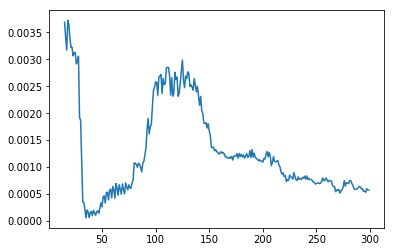
\includegraphics[width=12cm]{16.png}
          \caption{MyImprovedDQN:MountainCar-v0 loss曲线}
          \label{fig:2.3}
    \end{figure}
    \end{center}
    \begin{center}
    \begin{figure}[H]
          \centering
          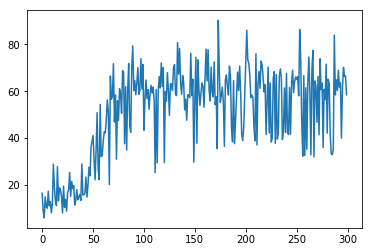
\includegraphics[width=12cm]{17.png}
          \caption{MyImprovedDQN:MountainCar-v0 sum of reward曲线}
          \label{fig:2.3}
    \end{figure}
    \end{center}
    \begin{center}
    \begin{figure}[H]
          \centering
          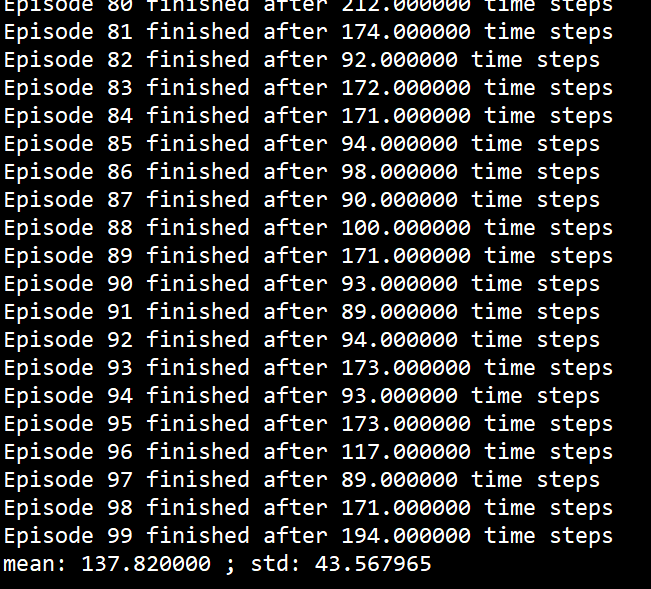
\includegraphics[width=12cm]{18.png}
          \caption{MyImprovedDQN:MountainCar-v0}
          \label{fig:2.3}
    \end{figure}
    \end{center}
    \subsection{Acrobot-v1}
    训练过程中损失(loss)变化如图19所示,累计奖赏(sum of reward)变化如图20所示。实验运行结果如图21所示。
    \begin{center}
    \begin{figure}[H]
          \centering
          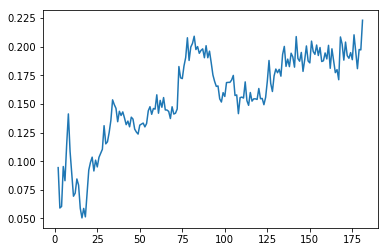
\includegraphics[width=12cm]{25.png}
          \caption{MyImprovedDQN:Acrobot-v1 loss曲线}
          \label{fig:2.3}
    \end{figure}
    \end{center}
    \begin{center}
    \begin{figure}[H]
          \centering
          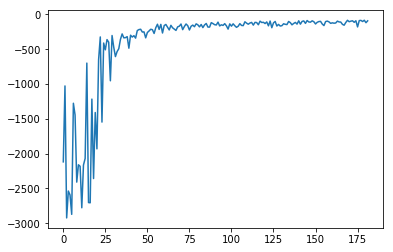
\includegraphics[width=12cm]{26.png}
          \caption{MyImprovedDQN:Acrobot-v1 sum of reward曲线}
          \label{fig:2.3}
    \end{figure}
    \end{center}
    \begin{center}
    \begin{figure}[H]
          \centering
          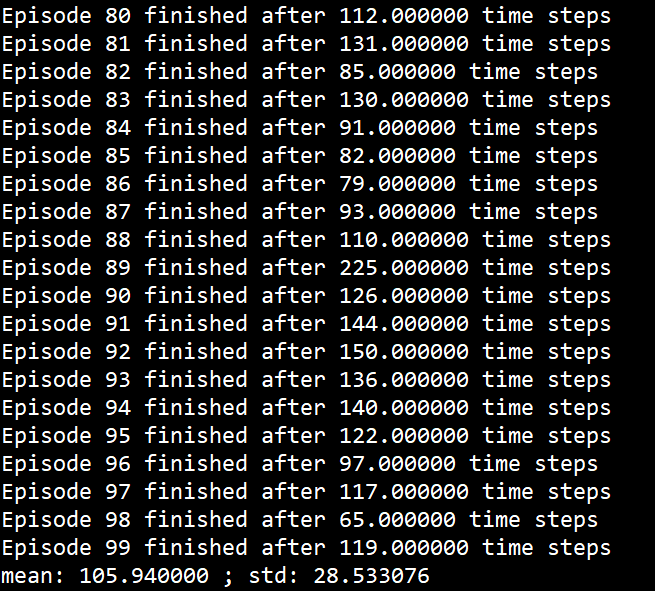
\includegraphics[width=12cm]{27.png}
          \caption{MyImprovedDQN:Acrobot-v1}
          \label{fig:2.3}
    \end{figure}
    \end{center}
    
\section{调参过程.}
    \paragraph*{}
    本部分按照介绍各个实验具体的调参过程中的问题和解决方式。	

    \subsection{实验二.MyQlearning}
    主要问题就是把各个连续状态空间划分为合适的区间。本实验采用的是等分的方式,未修改奖赏(reward)。因此主要方法就是比较笨的尝试几组参数,然后选择一个较好的,因此两个任务分别是(20,20)和(6,6,6,6,6,6)。
    比较奇怪的四第一个任务划分(1,1,6,5),因为发现前两个维度的划分会使实验效果下降,而最后一个维度取5和6差别很大,可能是因为区间划分的奇偶性以及状态的数量对该实验的收敛性有所影响。
    
    \subsection{实验三.MyDQN}
    主要问题是发现如果不修改奖赏算法很难收敛,或者训练过程中表现收敛但是测试时发现和没有训练没什么区别(比如任务三)。考虑到网络的结构为全连接层构成的MLP,各层均为线性,因此感觉上输入的状态以及输出的奖励都应该是
    连续的能反应实际情景的变量,因此对于三个任务,都修改了每一步的奖赏(reward),对于任务三,还重新定义了状态空间。具体如下:
    \begin{itemize}
    \item[-] 任务一的奖赏设为cartpole的角度和位置偏离中心的程度。
    \item[-] mountaincar设置为其小车相对底部的高度,高度越大,奖赏越大。
    \item[-] 通过阅读任务三的源代码,发现其状态空间各的分别是杆件一的角度的正余弦,杆件二相对于杆件一的角度的正余弦以及两者的角速度。其终止条件是两个杆件的高度之和大于1,因此修改奖励为两个杆件的高度之和,并输入状态为
    两个杆件的绝对角度的正弦和余弦值。
    \end{itemize}
    \subsection{实验四.MyImprovedDQN}
    和实验三参数基本一致。不同的是多了一个网络更新参数,在此统一设置为300。
    
\section{实验对比.}

    \begin{itemize}
    
    \item[-] 从训练程度上,实验二的训练轮数基本在两千步到三千步,而实验三和四的训练轮数基本在两百步到三百步。
    \item[-] 从训练结果上,有实验运行结果截图可以看出实验三四的效果明显好于实验二。实验三和四的差别不大,实验四略微好点。
    \item[-] 从稳定性上,实验二的运行非常稳定,结果基本可以复现;实验三和四的网络训练存在很多不稳定性训练,可能需要运行几次才能复现报告的结果。
    
    \end{itemize}
    
\end{document} 